\documentclass[12pt,a4paper]{article}
\pagestyle{plain}
\usepackage{fullpage}
\usepackage[english]{babel}
\usepackage{enumerate}

%equations
\usepackage[fleqn]{amsmath}
\numberwithin{equation}{section}

%figures
\usepackage[dvips]{graphicx}
\graphicspath{{./images/}}
\numberwithin{figure}{section}

%excercises
\newcounter{Exercise}
\setcounter{Exercise}{1}
\usepackage[dvipsnames]{xcolor}
\usepackage{framed}
\definecolor{shadecolor}{gray}{0.9}
\usepackage{caption}

%tables
\numberwithin{table}{section}

%specials
\usepackage{textcomp} %special (greek) characters as text
%\usepackage{pstricks} %
%\usepackage{ifthen} %
%\usepackage{calc} %
%\usepackage{isotope}
\usepackage{hyperref}
\usepackage[bottom]{footmisc} %footnote below figure
\usepackage{footnpag}%number footnotes per page


%document details
\author{N.G. Schultheiss \\ translated and adapted by K. Schadenberg}
\date{}
\title{Introduction Cosmic Radiation}


\begin{document}
\maketitle

\section{Introduction}
In the modules `The Sun' and `Solar Winds' we saw that our Sun is continuously sending particles into outer space, the Solar winds. There are two distinct groups of particles in these winds, low energetic particles coming from the poles and high energetic particles coming from Sun spots. Other stars in the universe are expected to emit particles with similar amounts of energy. When we look at figure~\ref{fig:spectrum} we see that there are particles with much higher energies present in cosmic rays. Where do these particles come from?

\begin{figure}\begin{center}
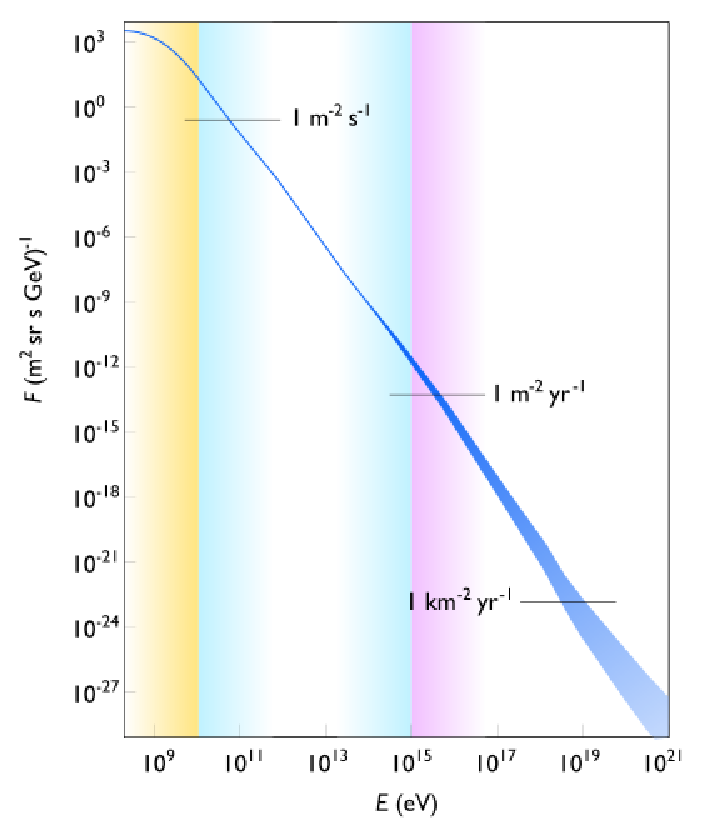
\includegraphics[scale=0.75]{Cosmic_ray_flux_versus_particle_energy.svg.eps}%
\caption{Energy spectrum of cosmic rays hitting the Earth.}\label{fig:spectrum}
\end{center}\end{figure}

\section{Sources of Cosmic Radiation}
\subsection{Stars}
The particles emitted by (normal) stars have a relative low energy. Can these low energy particles pick up speed/energy somewhere in the universe?

The behaviour of moving electric charges in magnetic fields has been described in the module `Solar Winds'. The particles feel a magnetic force, part of the Lorentz force, perpendicular to the field and their direction of travel. In a uniform field the particles will be deflected from their straight path, but the speed does not increase. In a divergent field however the speed of the particles does increase. If there is a strong (or strongly) divergent divergent field somewhere in the universe then this could (partly) explain the energy spectrum of figure~\ref{fig:spectrum}. Low energy particles emitted by stars pick up speed (energy) when they travel through the magnetic field.

\subsection{Black Holes \& Supernovae}
Magnetic field could explain the spectrum of figure~\ref{fig:spectrum}, but where are these fields? What kind of phenomena could create these strong fields? Are there perhaps other celestial bodies which emit high energy radiation? Two possible sources of both high energy particles and strong divergent magnetic fields are black holes and supernovae.

\begin{shaded}
\textbf{Exercise \theExercise \stepcounter{Exercise}} : What can you say about the intensity\footnotemark of cosmic radiation coming from black holes?

What can you say about the (minumum) amount of energy of particles emitted by black holes?\end{shaded}
\footnotetext{As always in physics, we must be very careful in the words we choose and their meaning. Intensity is a measure of (average) energy flux, the amount of energy flowing through a fixed area per second.}

\begin{shaded}
\textbf{Exercise \theExercise \stepcounter{Exercise}} : How would you describe the radiation coming from a supernova? Use the word intensity in your description. Is this intensity constant over time?\end{shaded}

Supernovae are very violent events, fortunately there are no stars in danger of going nova in close proximity to the Earth. If a nearby star were to explode as a supernova then life on Earth would almost certainly cease to be.

Lets take a look at a hypothetical supernova 100~light~year away, far away but still `close by' on the scale of the entire universe. The protons emitted by this explosion have an energy 100~GeV.
\begin{shaded}
\textbf{Exercise \theExercise \stepcounter{Exercise}} : What is the difference in arrival times of the photons (light) and protons emitted by our hypothetical supernova? Is the answer you obtained realistic?\end{shaded}

In answering the previous question you probably calculated the speed of the proton using the formula for kinetic energy $E=\frac{1}{2}mv^2$. In doing so you obtained a speed higher than the speed of light, something which is impossible. We need to take into account relativity and the famous equations of Albert Einstein, $E=mc^2$. Relativity is discussed in more detail in the module `Relativity'. For now we will simply state the equations we need to use:
\begin{align}
& E=\gamma mc^2 \label{eq:energy}\\
& \gamma = \frac{1}{\sqrt{1-\left( \frac{v}{c} \right)^2 }} \label{eq:lorentz}
\end{align}
$\gamma$ is known as the gamma or Lorentz factor. Normal SI units can be used with these equations. However, in particle physics the mass of usually denoted in $\frac{\mbox{MeV}}{c^2}$. When we use this unit in equation~\ref{eq:energy} we immediately obtain an energy in eV.

The proton has a mass of $938.3~\frac{\mbox{MeV}}{c^2}$, using this in equations~\ref{eq:lorentz} and \ref{eq:energy} yields:
\begin{align}
E &= \frac{1}{\sqrt{1-\left( \frac{v}{c}\right)^2}} mc^2 \\
100~\mbox{GeV} &= \frac{1}{\sqrt{1-\left( \frac{v}{c}\right)^2}} 938.3~\frac{\mbox{GeV}}{c^2}c^2 \\
100~\mbox{GeV} &= \frac{1}{\sqrt{1-\left( \frac{v}{c}\right)^2}} 938.3~\mbox{GeV} \\
\frac{100000}{938.3} &= \frac{1}{\sqrt{1-\left( \frac{v}{c}\right)^2}} \\
0.09669 &= 1 - \left( \frac{v}{c} \right)^2 
\end{align}
\begin{align}
\left( \frac{v}{c} \right)^2 &= 1-0.09669=0.90331 \\
\frac{v}{c} &= 0.95043 \\
v &= 0.95043~c
\end{align}

Light covers a distance of 100~light~year in 100 years. Protons take a factor $\frac{1}{0.95043}$ longer to travel the same distance, i.e. they need $\frac{100}{0.95043}=105.22~\mbox{years}$.

\begin{shaded}
\textbf{Exercise \theExercise \stepcounter{Exercise}} : How far behind the light do protons with an energy of 1000~GeV arrive if they came from our hypothetical supernova?\end{shaded}

\section{Fields in Space}
In the module `The Expanding Universe' we saw that the Andromeda nebula (actually a galaxy) is coming towards our galaxy, the Milky Way, with a speed of 300~km/s. Inside the Andromeda galaxy there are almost certainly different electromagnetic fields. These fields travel towards us with the same speed. All charged particles inside Andromeda will feel a Lorentz force.

What is the effect of this force? Lets take a look at a a stationary magnetic field and a proton moving towards the field with a speed of 300~km/s.\footnote{This situation is nearly the same are the reverse; a moving field and a stationary particle. However, a changing magnetic field introduces an electrical field, complicating the calculation we want to show here.} The path of the proton is shown in figure~\ref{fig:field}. The velocity of the particle is reversed, the field acts like a `magnetic mirror'.

Lets expand the previous example by giving the magnetic field a speed of 300~km/s towards the proton. In the lab frame (us as stationary observers a long way away) we have a proton with speed 300~km/s and a field with speed $-300$~km/s. In the cloud frame (from the point of view of the field as being stationary) the only thing moving is the proton with a speed of 600~km/s. After the collision of the proton and the field the new velocity of the proton is -600~km/s. But in the lab frame this is $-(300+300)-300 = 900$~km/s! Of course this calculation is only valid when the speeds remain far below the speed of light.

\begin{figure}\begin{center}
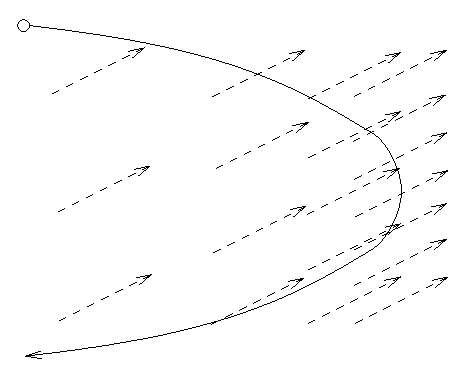
\includegraphics[scale=1]{field.eps}%
\caption{Moving charged particle encountering a static magnetic field. The field acts like a mirror reversing the velocity of the particle.}\label{fig:field}
\end{center}\end{figure}

\begin{shaded}
\textbf{Exercise \theExercise \stepcounter{Exercise}} : Are photons affected by electromagnetic fields? Why, or why not?\end{shaded}
\begin{shaded}
\textbf{Exercise \theExercise \stepcounter{Exercise}} : What happens more frequently: a head on collision between a charged particle and a magnetic field, or a particle trying to overtake a magnetic field? Why?

Hint: When you cycle on a two-way bicycle path, do you encounter more oncoming traffic or are you overtaking more other cyclists travelling in the same direction?
\end{shaded}
\begin{shaded}
\textbf{Exercise \theExercise \stepcounter{Exercise}} : Does the difference in arrival times of protons and photons change because of (moving) magnetic fields? If so, does the difference increase or decrease?

Hint: What happens when a proton collides with a magnetic field moving away from the proton, i.e. what happens when a proton tries to overtake a magnetic field?\end{shaded}
\begin{shaded}
\textbf{Exercise \theExercise \stepcounter{Exercise}} : Does the direction from where cosmic rays hit the Earth tell us anything about the direction of travel of the source?\end{shaded}

\end{document}
